% !TEX encoding = UTF-8 Unicode
\documentclass[a4paper]{article}

\usepackage{color}
\usepackage{url}
\usepackage[T2A]{fontenc} % enable Cyrillic fonts
\usepackage[utf8]{inputenc} % make weird characters work
\usepackage{graphicx}
\usepackage{mathtools}
\usepackage{amsmath}
\usepackage[english,serbian]{babel}
\usepackage{comment}
\usepackage{multirow}
\usepackage[svgnames,table]{xcolor}
\usepackage{tikz}
\usepackage{longtable}
\usepackage{changepage}
\usepackage{setspace}
\usepackage{hhline}
\usepackage{multicol}
\usepackage{tabto}
%\usepackage[english,serbianc]{babel} %ukljuciti babel sa ovim opcijama, umesto gornjim, ukoliko se koristi cirilica

\usepackage[unicode]{hyperref}
\hypersetup{colorlinks,citecolor=green,filecolor=green,linkcolor=blue,urlcolor=blue}

\usepackage{listings}

%\newtheorem{primer}{Пример}[section] %ćirilični primer
\newtheorem{primer}{Primer}[section]

\definecolor{mygreen}{rgb}{0,0.6,0}
\definecolor{mygray}{rgb}{0.5,0.5,0.5}
\definecolor{mymauve}{rgb}{0.58,0,0.82}

\lstset{ 
  backgroundcolor=\color{white},   % choose the background color; you must add \usepackage{color} or \usepackage{xcolor}; should come as last argument
  basicstyle=\scriptsize\ttfamily,        % the size of the fonts that are used for the code
  breakatwhitespace=false,         % sets if automatic breaks should only happen at whitespace
  breaklines=true,                 % sets automatic line breaking
  captionpos=b,                    % sets the caption-position to bottom
  commentstyle=\color{mygreen},    % comment style
  deletekeywords={...},            % if you want to delete keywords from the given language
  escapeinside={\%*}{*)},          % if you want to add LaTeX within your code
  extendedchars=true,              % lets you use non-ASCII characters; for 8-bits encodings only, does not work with UTF-8
  firstnumber=1000,                % start line enumeration with line 1000
  frame=single,	                   % adds a frame around the code
  keepspaces=true,                 % keeps spaces in text, useful for keeping indentation of code (possibly needs columns=flexible)
  keywordstyle=\color{blue},       % keyword style
  language=Python,                 % the language of the code
  morekeywords={*,...},            % if you want to add more keywords to the set
  numbers=left,                    % where to put the line-numbers; possible values are (none, left, right)
  numbersep=5pt,                   % how far the line-numbers are from the code
  numberstyle=\tiny\color{mygray}, % the style that is used for the line-numbers
  rulecolor=\color{black},         % if not set, the frame-color may be changed on line-breaks within not-black text (e.g. comments (green here))
  showspaces=false,                % show spaces everywhere adding particular underscores; it overrides 'showstringspaces'
  showstringspaces=false,          % underline spaces within strings only
  showtabs=false,                  % show tabs within strings adding particular underscores
  stepnumber=2,                    % the step between two line-numbers. If it's 1, each line will be numbered
  stringstyle=\color{mymauve},     % string literal style
  tabsize=2,	                   % sets default tabsize to 2 spaces
  title=\lstname                   % show the filename of files included with \lstinputlisting; also try caption instead of title
}

\begin{document}

\title{Razvoj rekurentne neuronske mreže i primena na analizi vremenskih serija\\  \small{Seminarski rad u okviru kursa\\Računarska inteligencija\\ Matematički fakultet}}

\author{Kristina Pantelić, 91/2016, kristinapantelic@gmail.com \\Nevena Mesar, 107/2015, @.com }

%\date{.}

\maketitle

\abstract{
Danas je upotreba neuronskih mreža za rešavanje diverziteta računarskih problema u širokoj upotrebi. Za različite probleme koriste se različite vrste neuronskih mreža. U ovom radu čitalac će se upoznati sa terminom neurona, neuronske mreže, rekurentne neuronske mreže i primenom rekurentne neuronske mreže na analizi vremenskih serija.
}

\tableofcontents

\newpage

\section{Uvod}
\label{sec:uvod}

Algoritmi neuronskih mreža su nastali kao pokušaj da se oponaša način na koji ljudski
mozak uči tj. način na koji ljudski mozak klasifikuje i spoznaje stvari. Neuronske mreže su razvijene tako da simuliraju neurone tj. mreže neurona mozga\cite{master_rad}. U tradicionalnoj neuronskoj mreži svi ulazi i izlazi su nezavisni jedni od drugih, ali u slučajevima kada se, na primer, zahteva predviđanje sledeće reči u rečenici, zahteva se da imamo informaciju o prethodnoj reči i da je na neki način zapamtimo\cite{introRNN}. Ovaj problem je bio motivacija za pojavljivanje i razvijanje rekurentne neuronske mreže. Rekurentna neuronska mreža (RNN) ima "memoriju"{} koja pamti sve informacije koje je prethodno izračunala tj. naučila. Treba imati na umu da tradicionalna neuronska mreža takođe pamti informacije, ali samo one koje je naučila tokom treninga. Na primer, ako klasifikator nauči zavisnosti ulaznih od izlaznih podataka tokom treninga, koristiće to znanje da klasifikuje test instance. Dok RNN takođe uči prilikom treninga, dodatno, ona pamti informacije naučene iz prethodnih trening instanci da bi generisala izlazne podatke\cite{introRNN2}. Ovo svojstvo pamćenja informacija kroz vreme omogućava RNN mreži predikciju u oblasti vremenskih serija\cite{introRNN}, kojima u ovom radu posvećujemo pažnju u kontekstu primene RNN. \\
\indent Na samom početku ovog rada upoznaćemo se sa modelom naše rekurentne neuronske mreže, a u daljem tekstu ćemo se upoznati sa korišćenim skupom podataka vremenskih serija i primenom RNN na skup.  


\section{Rekurenta neuronska mreža}
\label{sec:model}

Postoji više vrsta neuronskih mreža koja, svaka zbog svojih specifičnih karakteristika, daju dobre rezultate na specifičnim poljima istraživanja podataka. Vrsta mreže koja je tema našeg rada je rekurentna neuronska mreža, a naša koncentracija je na razvijanju Jordanove strukturne rekurentne neuronske mreže (eng. \textit{Jordan SRNN}).\\
\indent Jordanova rekurentna neuronska mreža je zasnovana na konceptu koji podrazumeva ponovno korišćenje dobijenih izlaznih vrednosti mreže kao dodatnih informacija za usmeravanje pretrage i izračunavanje novih vrednosti rezultata. Pored ulaznih instanci, dodaju se novih $k$ vrednosti koje predstavljaju vrednosti $k$ rezultata. Dakle, kopija izlaznog sloja se sprovodi na ulaz.\\
%Rekurentna neuronska mreža kojoj posvećujemo pažnju je Jordanova rekurentna neuronska mreža. 
\indent Naš cilj je konstruisati rekurentu neuronsku mrežu sa jednim skrivenim slojem koja će za 6 unetih uzastopnih dana prognozirati količinu padavina za 7. dan. U nastavu ćemo predstaviti model ove mreže u skladu sa brojem naših izlaznih vrednosti (jedan izlazni podatak) i odgovarajuće oznake korišćene u k\^{o}du za implementaciju mreže.

\subsection{Model rekurentne neuronske mreže}
\label{sec:model}

Neuronska mreža se sastoji od 3 sloja koju čine ulazni, skriveni i izlazni sloj. Svaki od slojeva ima odgovarajući broj neurona tj. promenljivih.
Ulazni sloj se sastoji od $n+p$ ulaznih promenljivih $x^{(l)}_1$, $x^{(l)}_2$, ..., $x^{(l)}_n$,$o^{(l-1)}_1$, $o^{(l-1)}_2$, …, $o^{(l-1)}_p$,  uz dodatnu promeljivu $x^{(l)}_0$, koja se naziva bajes i čija je vrednost uvek jednaka 1, za svako $l$. Promenljiva $l$ u superskriptu promenljive $x_i$ predstavlja redni broj instance u skupu odabranih instanci za treniranje mreže. Radi jednostavnosti sve ulazne promenljive označavamo sa $x_i {}\in{}[ \,0,n+p ] \,$. Skriveni sloj čine $m$ neurona $h^{(l)}_1$, $h^{(l)}_2$, …, $h^{(l)}_m$ uz dodatnu promenljivu $h^{(l)}_0=1$, za svako $l$, koja predstavlja bajes za skriveni sloj mreže. Izlazni sloj čine $p$ neurona, čiji su izlazi $o^{(l)}_1$, $o^{(l)}_2$, …, $o^{(l)}_p$. Svi neuroni ulaznog sloja su spojeni sa svim neuronima skrivenog sloja, osim bajesa, vezama čije su težine $w’_{ij}$, $0\leq{}i\leq{}n+p$, $0\leq{}j\leq{}m$. Svi neuroni skrivenog sloja su povezani sa svim neuronima izlaznog sloja vezama sa težinama $w{''}_{jk}$, $0\leq{}j\leq{}m$, $1\leq{}k\leq{}p$. 

Nakon završavanja algoritma, cilj je da izlazne vrednosti budu što bliže izlaznim vrednostima $y_1$, $y_2$,...,$y_p$.

\begin{figure}[h!]
\begin{center}
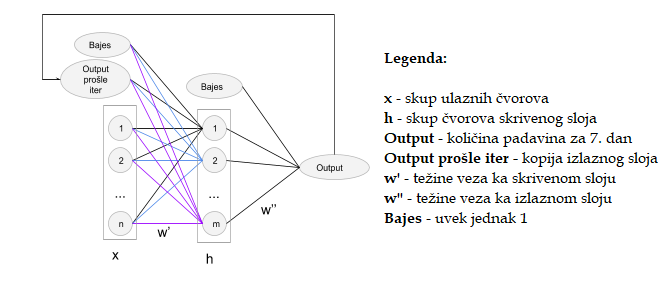
\includegraphics[scale=0.7]{net.png}
\end{center}
\caption{Jordanova RNN sa jednim skrivenim slojem}
\end{figure}

Proces učenja se sastoji od više iteracija, gde se svaka iteracija izvršava u nekoliko koraka. Najpre se, za sve $j$, $1\leq{}j\leq{}m$, izračunava vrednost:

\begin{equation}
u'_j = \sum_{i=0}^{n+p}x_iw'_{ij}
\end{equation}
 
i $h_j= f(u'_j)$, gde je $f(x)=(1+e^{-x})^{-1}$ sigmoidna funkcija. Sigmoidna funkcija predstavlja aktivacionu funkciju neurona skrivenog i izlaznog sloja. Analogno kao kod skrivenog sloja, određuju se vrednosti izlaza iz neurona izlaznog sloja. Tako se dobija 

\begin{equation}
u{''}_k = \sum_{ij=0}^{m}h_jw{''}_{jk}
\end{equation}
 
i $o_k= f(u{''}_k)$. Nakon odgovarajućeg broja iteracija, očekujemo da će vrednosti $o_k$ biti približno jednake željenim izlaznim vrednostima $y_k$.
Greška izlaznog sloja neurona k je definisana:

\begin{equation}
E_k = \frac{1}{2}(y_k - o_k)^2.
\end{equation}

Pri ažuriranju vrednosti $w{''}_{jk}$, važi $w{''}_{jk}=w{''}_{jk}+w{''}_jk$, gde je
$$\Delta{} w{''}_{jk}=- \eta{}\frac{\partial{}E_k}{\partial{}w{''}_{jk}}+\alpha{}w{''}_{jk}.$$

Parametri $\eta{}$ i $\alpha{}$, respektivno, mere uticaj parcijalnog izvoda greške $E_k$ po $w{''}_{jk}$ i prethodne vrednosti $w{''}_{jk}$. Kako je $E_k$ funkcija od $o_k$, $o_k$ funkcija od $u{''}_k$, a $u{''}_k$ funckija čiji je jedan od argumenata $w{''}_{jk}$, prema pravilu o izvodu složene funkcije važi 

$$\frac{\partial{}E_k}{\partial{}w{''}_{jk}} = \frac{\partial{}E_k}{\partial{}o_{k}}\frac{\partial{}o_k}{\partial{}u{''}_{k}}\frac{\partial{}u{''}_k}{\partial{}w{''}_{jk}} = -(y_k-o_k)f'(u{''}_k)h_j = -(y_k-o_k)o_k(1-o_k)h_j$$

Iz poslednjeg reda sledi da je 

$$\Delta{}w{''}_{jk}=\eta{}(y_k-o_k)o_k(1-o_k)h_j+\alpha{}w{''}_{jk}$$

Greška neurona skrivenog sloja predstavlja sumu svih odgovarajućih grešaka neurona izlaznog sloja i određena je sa

$$E_j = \frac{1}{2}\sum_{k=1}^p(y_k - o_k)^2$$.

Pri ažuriranju vrednosti $w'_{ij}$, važi $w'_{ij}=w'_{ij} + \Delta{}w'_{ij}$, gde je

$$\Delta{}{}w'_{ij} = - \eta{}\frac{\partial{}E_j}{\partial{}w{'}_{ij}}+\alpha{}w'_{ij}$$.

Vrednost $\frac{\partial{}E_j}{\partial{}w'_{ij}}$ se može izračunati prema pravilu o izvodu složene funkcije na sledeći način:

$$\frac{\partial{}E_j}{\partial{}w'_{ij}}=\frac{\partial{}E_j}{\partial{}o_{k}}\frac{\partial{}o_k}{\partial{}u{''}_{k}}\frac{\partial{}u{''}_k}{\partial{}h_{j}}\frac{\partial{}h_j}{\partial{}u'_{j}}\frac{\partial{}u'_j}{\partial{}w'_{ij}}$$
$$ = -\sum_{k=1}^p(y_k-o_k)f'(u{''}_k)w{''}_{jk}f'(u'_j)x_i$$
$$ = -\sum_{k=1}^p(y_k-o_k)o_k(1-o_k)w{''}_{jk}h_j(1-h_j)x_i$$

Sledi da je 
$$\Delta{}w'_{ij}=\eta{}x_ih_j(1-h_j)\sum_{k=1}^p(y_k-o_k)o_k(1-o_k)w{''}_{jk} + \alpha{}\Delta{}w'_{ij}\cite{model}$$

\subsection{Algoritam rekurentne neuronske mreže}
\label{sec:model}

Na osnovu prethodnog opisa, algoritam učenja se izvršava u sledećih osam koraka\cite{model}:

\begin{enumerate}
  \item Ulazni podaci se sastoje od parova vektora ($x^{(l)}_1$, $x^{(l)}_2$,..., $x^{(l)}_{n+p}$) i ($y_1$, $y_2$,..., $y_p$), gde $x_i$ predstavljaju ulaze uključujući kopiju rezultata iz prethodne iteracije algoritma, a $y_k$ željene izlaze za svaku ulaznu instancu. Skup ulaznih podataka se proširuje bajesom $x^{(l)}_0=1, {}\forall{l}$ iz skupa podataka.
  \item Inicijalizovati parametre $\eta{}$, $\alpha{}$ i odrediti kriterijum zaustavljanja. Inicijalizovati početne vrednosti za $w'_{ij}$ i $w{''}_{jk}$ i postaviti $\Delta{}w'_{ij}=\Delta{}w{''}_{jk}=0$. Izabrati aktivacionu funkciju f (ovde je korišćena sigmoidna funkcija).
  \item Izabrati novi par ulaznog i izlaznog vektora (novi test primer iz skupa za učenje).
  \item Odrediti vrednosti $u'_j$ i $h_j$. Postaviti $h^{(l)}_0=1, {}\forall{l}$ iz skupa podataka.
  \item Odrediti vrednosti $u{''}_k$ i $o_k$. Ukoliko je ispunjen kriterijum zaustavljanja, prekinuti izvršavanje.
  \item Odrediti $\Delta{}w{''}_{jk}$ i ažurirati vrednosti $w{''}_{jk}$.
  \item Odrediti $\Delta{}w{'}_{ij}$ i ažurirati vrednosti $w{'}_{ij}$.
  \item Preći na korak 3.
\end{enumerate}

\addcontentsline{toc}{section}{Literatura}
\appendix
\bibliography{seminarski} 
\bibliographystyle{plain}

\appendix
\section{Dodatak}


\end{document}
